\section{Results \& Discussion}
In this chapter we summarize and give an overview of the results of Chapter \ref{sec:analysis} (Section \ref{sec:results}), discuss problems and assumptions throughout the work, strengthen the outcome of this thesis by showing our key plot again for actions calculated in a wrong calculated potential in Section \ref{sec:wrong_results} and give a future perspective in Section \ref{sec:discussion}.

\subsection{Signatures of \aclp{IMBH} in action space}\label{sec:results}
In Section \ref{sec:action_space} we got some clear differences between the simulations with and without \ac{IMBH}, and we took them as signatures of the \ac{IMBH}. For SIM 1, we juxtapose the three signature plots containing the radial actions and mark the stars of the different groups. Group 1 (yellow) includes the stars with high negative energies and low radial actions which are most likely bound or affected by the \ac{IMBH}. Group 2 (red) contains the stars having an total energy close to zero and high radial actions. These could be different to SIM 3 and SIM 4 only due to different truncation prescriptions since the stars are located in the outer region of the \acs{GC}. Group 3 (blue) contains all stars having a guiding-star radius below \unit[0.1]{pc}, that are only there for the simulations with \ac{IMBH}. 
\begin{figure}[htbp]
\centering
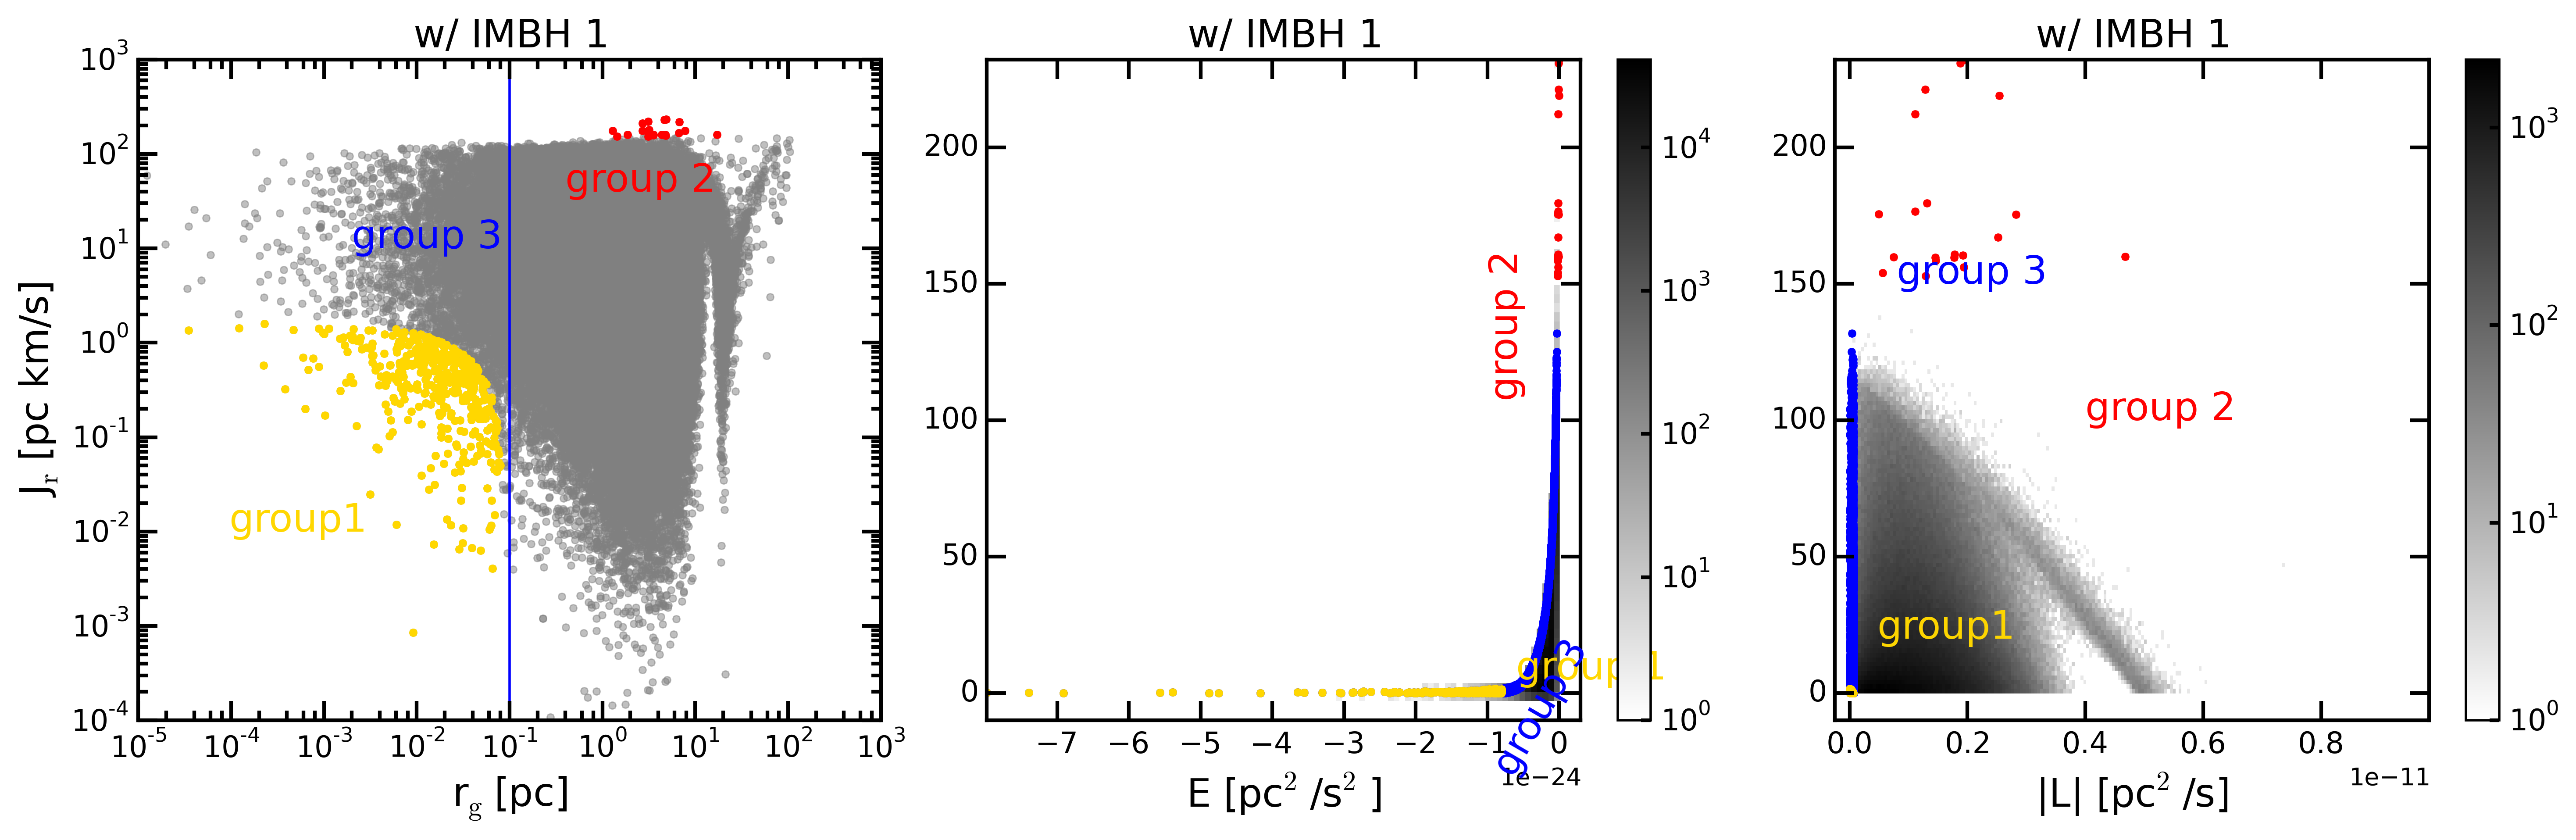
\includegraphics[width=\textwidth]{Plots/J_r_compare_plot.png}
\caption{Radial action over different values with marked groups of stars. In the first panel the radial action is plotted versus the guiding star radius, in the next panel as histogram over the energy and in the last panel as histogram over the angular momentum. Group 1 marked yellow includes all stars having an energy below \unitfrac[9$\times 10^-{25}$]{pc$^2$}{s$^2$}. Group 2 (red) marks all stars having a radial action over \unitfrac[150]{pc km}{s}. Group 3 in blue contains all stars having a guiding star radius below \unit[0.1]{pc}.}
\label{fig:J_r_compare}
\end{figure}
\par 
Figure \ref{fig:J_r_compare} is divided into three panels. In all panels the whole simulation is given in grey, in the second and third panel it is color coded with the number of the stars per bin. The different groups are color coded as mentioned above. In the first panel we see the different groups, their guiding-star radii and their radial actions. Group 1 is included in group 3 and is the part with the lowest radial actions. It has a clear round shape which could be another significant property. 
\par The second panel shows the histogram of the radial action over the energy. This is the plot where we can clearly see and select the stars of group 1 and group 2. Group 1 stars are on the bottom of the plot where the radial action is almost zero and the energy is very high. Group 2 stars are located at energies close to zero with high radial action. The stars of group 3 cannot be directly seen here. For each energy they have the highest occurring radial action and are located along the upper edge of the main shape which is best seen in Figures \ref{fig:E_J_r_hist_noIMBH1} and \ref{fig:E_J_r_hist_noIMBH1}. Since the stars of group 3 have only  small guiding-star radii they should not have far-off apocentres but they can have pericentres close to the black hole. Having the highest radial actions at given energies these stars have very eccentric orbits. 
\par The third plot is the radial action versus angular momentum histogram. Group 1 and group 3 stars cannot be distinguished from other stars in there, since given small guiding-star radius they have only a small angular momentum. There are many other stars not belonging to group 1 nor group 3 which have a very small angular momentum as well. Only stars of group 2 can be seen above a radial action of \unitfrac[150]{pc km}{s}. But this plot reveals something else: the mass dependency of the radial actions and the angular momentum. We clearly see a substructure from 0.3 until \unitfrac[0.6]{pc$^2$}{s} independent of all groups. In Figure \ref{fig:L_J_r_hist} we have seen that this substructure is due to the mass dependence. 
\par To summarize, stars in group 1 are a clear signature of a presence of an \ac{IMBH} and they can be detected as a tail at high energy in the radial action versus energy plot. These stars are indeed the closest to the \ac{IMBH} (small guiding star radius), and have very circular orbits. Therefore we interpret them as bound stars to the \ac{IMBH}. They are not observed in the simulations without \ac{IMBH}.


\subsection{Robustness of the results: using a wrong potential}\label{sec:wrong_results}
One test to re-check our results is to use a randomly wrong stellar mass density which is the basis of all our calculations. In Figure \ref{fig:wrong_phase_space}, we compare the right and the wrong density.
\begin{figure}[htbp]
\subcaptionbox{Density profiles of right and wrong density of SIM1. While the right density has a gentle gradient the wrong density exhibits a core profile in the central part and a steep gradient in the outer part. In the central part, the density is too low while in the outer part it is higher than the right one. \label{fig:wrong_density}}{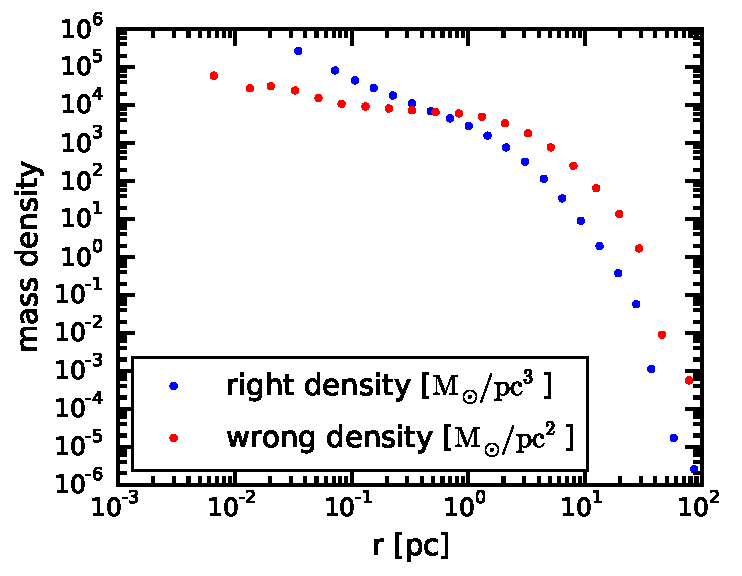
\includegraphics[width=0.47\textwidth]{Plots/wrong_density_profiles.pdf}}
\hfill
\subcaptionbox{Potential versus radius of right and wrong density of SIM1. The right potential has a steep gradient in the centre of the \ac{GC} and flattens rapidly. The wrong potential is always higher in absolute values and has a two step flattening. The first flattening is at the same distance as the one from the right potential but from there it is much higher than the right potential. The second flattening step is where the density profile starts falling rapidly. \label{fig:wrong_potential}}{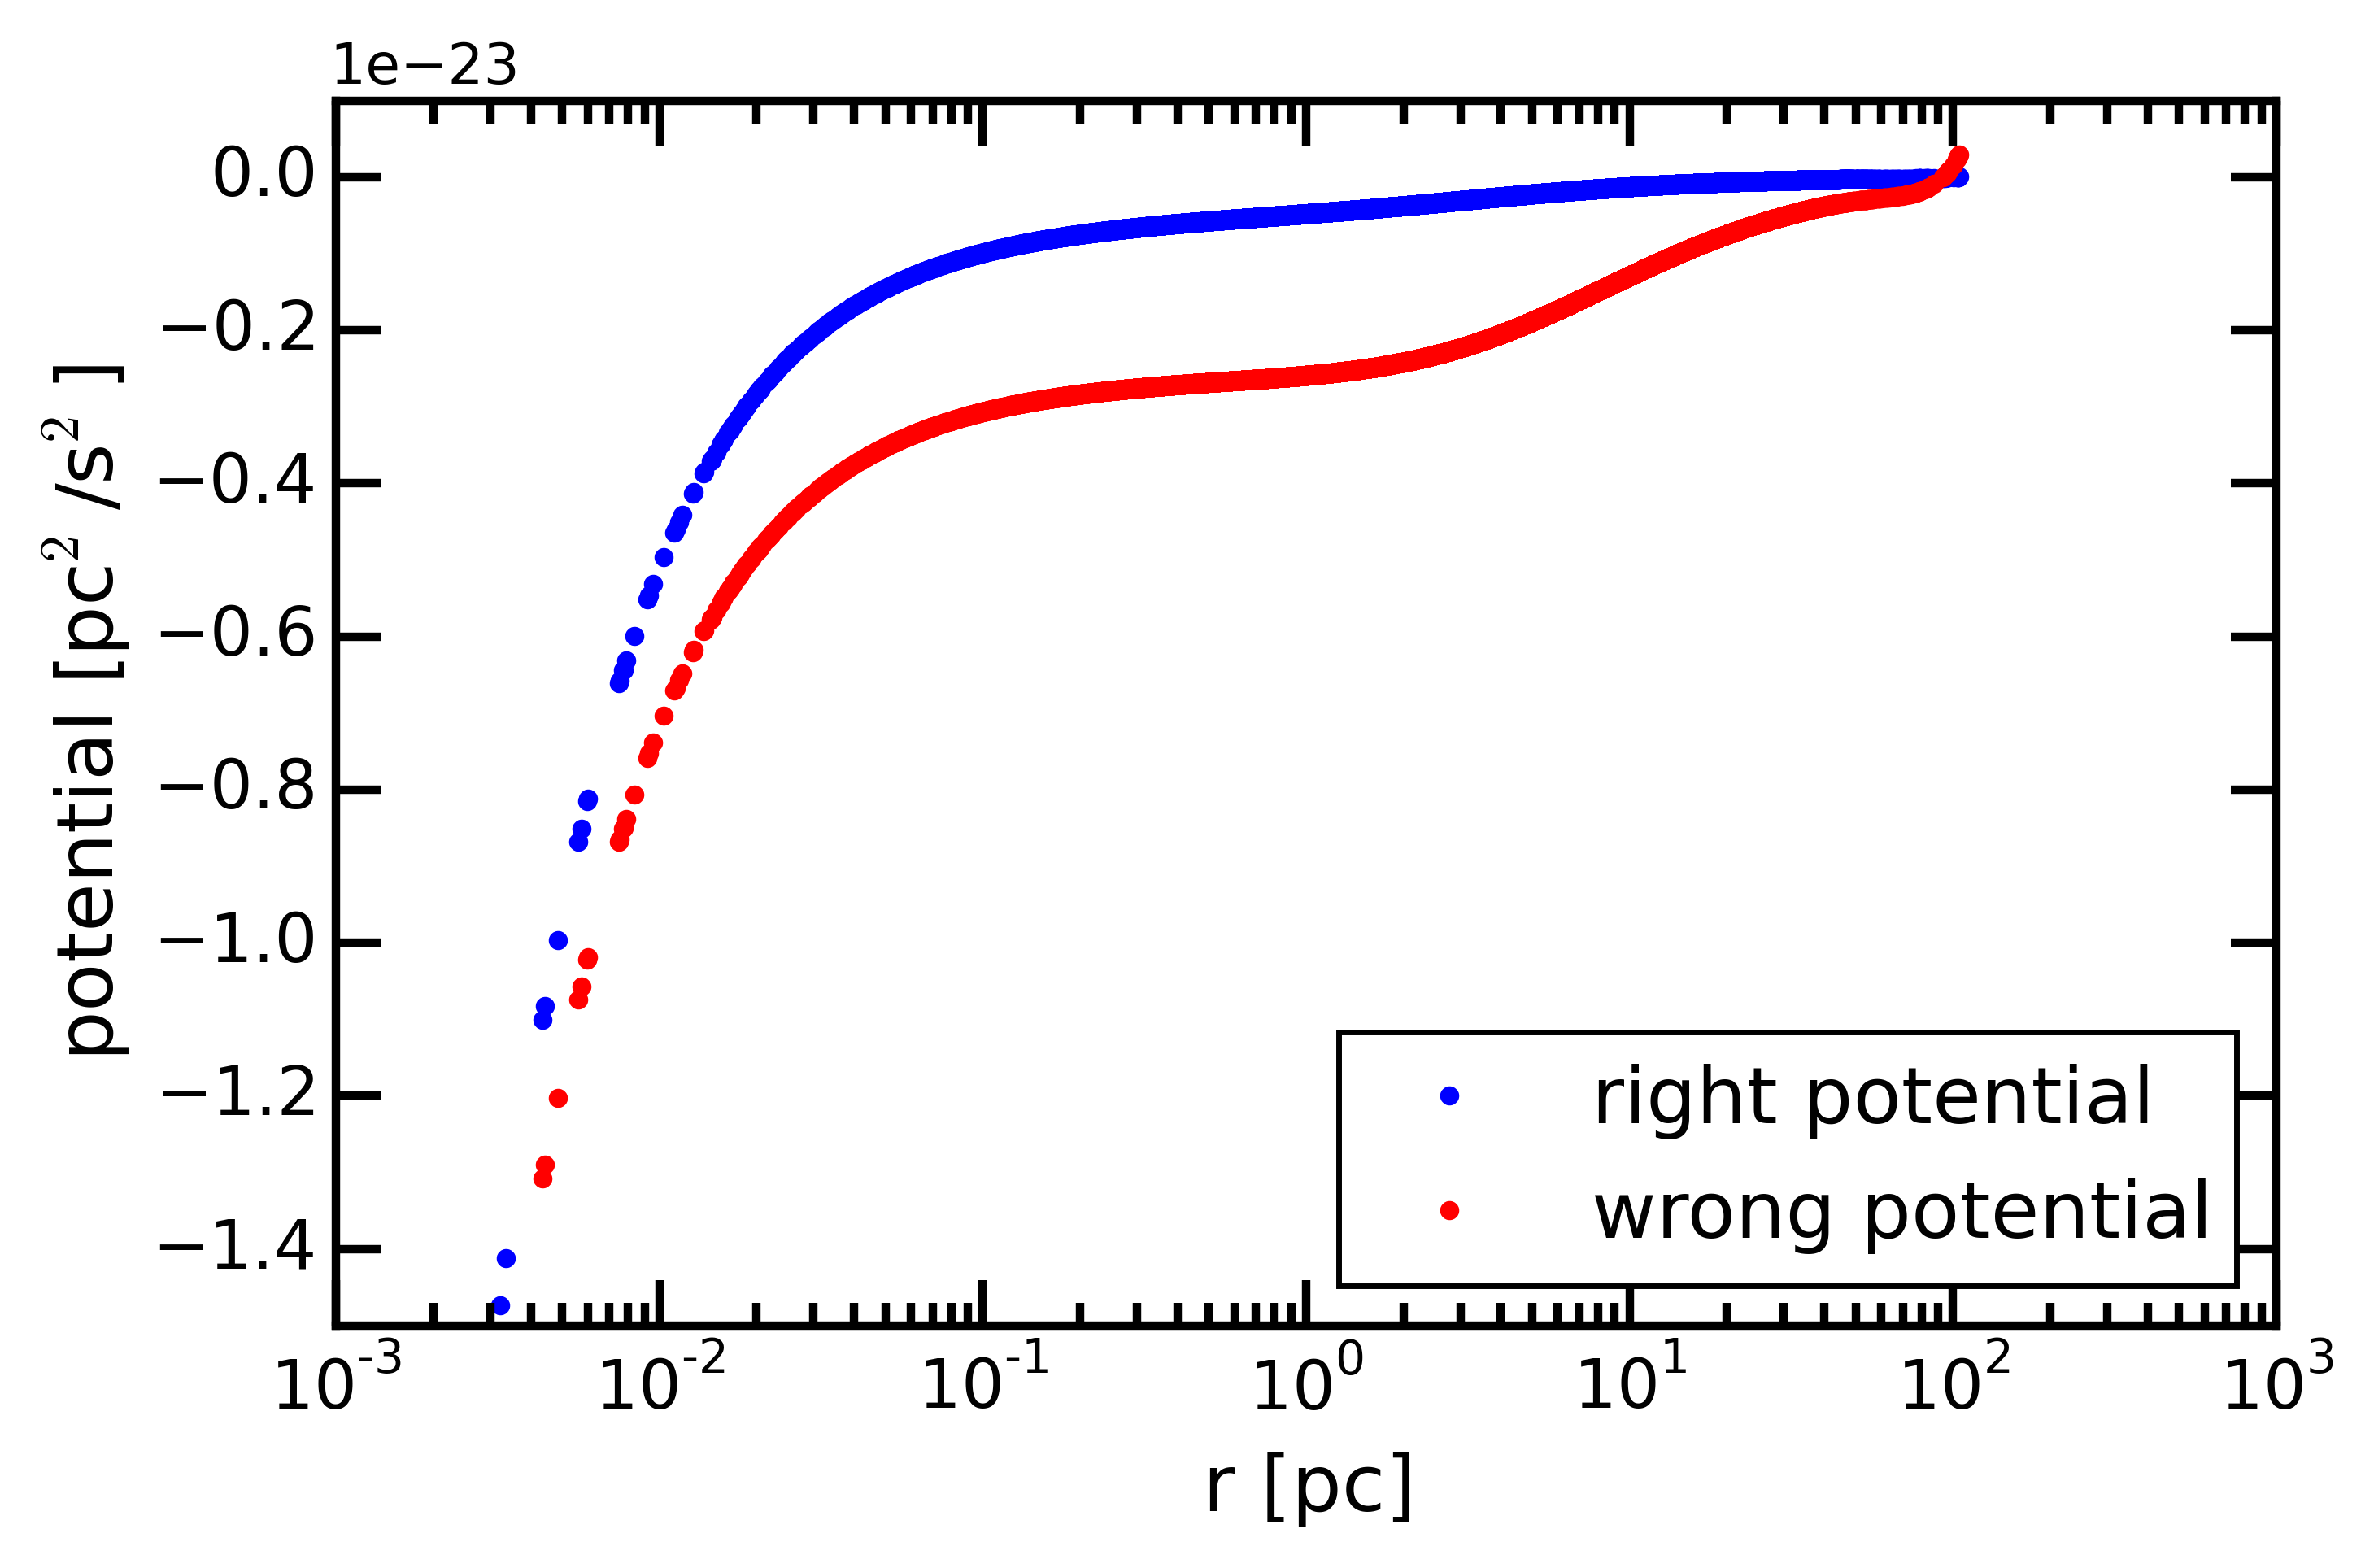
\includegraphics[width=0.48\textwidth]{Plots/wrong_potential.png}}
\caption{Comparison of right (blue) and wrong (red) calculated density and potential of SIM 1. }
\label{fig:wrong_phase_space}
\end{figure}

\par With this wrong potential we can also get the key plot from Section \ref{sec:results} given in Figure \ref{fig:J_r_compare_wrong}.
\begin{figure}[htbp]
\centering
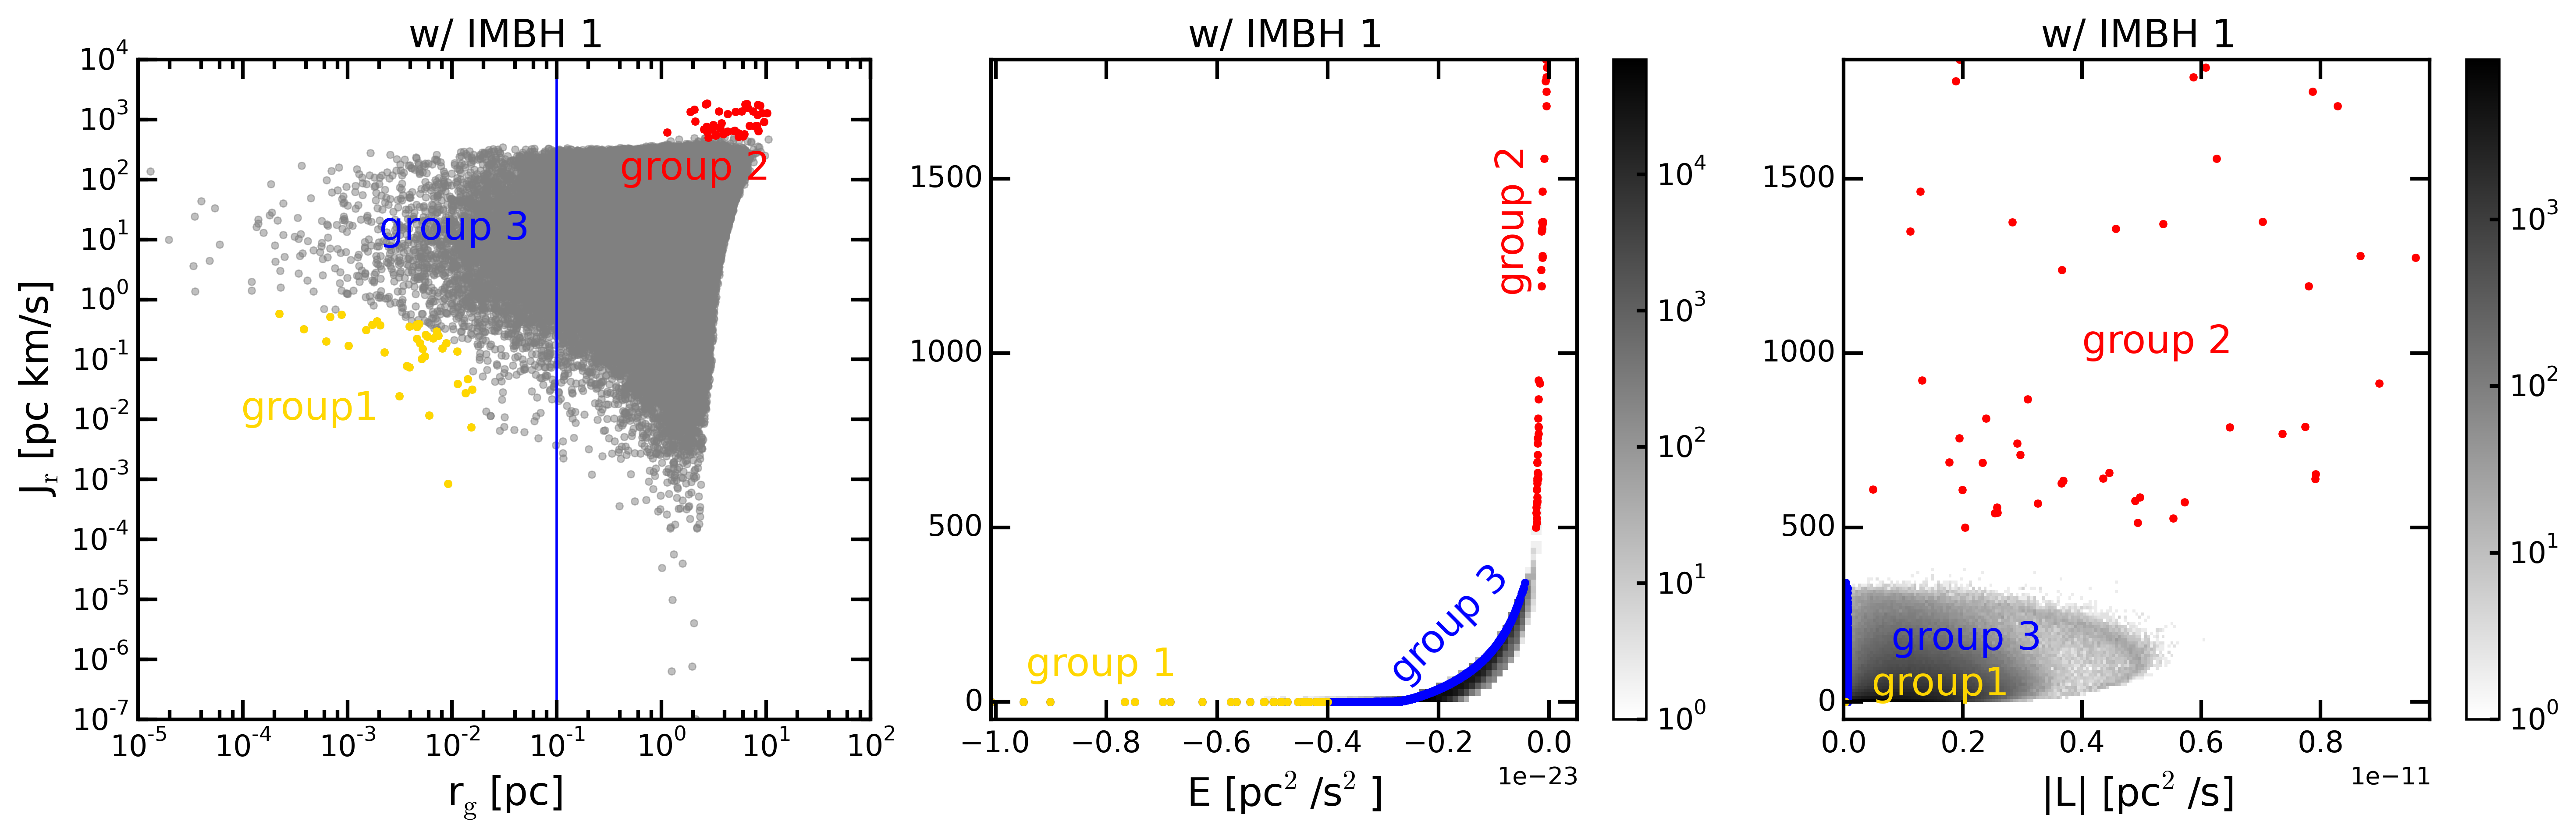
\includegraphics[width=\textwidth]{Plots/surface_density/J_r_compare_plot.png}
\caption{Radial action over guiding-star radius, energy and angular momentum, computed using a wrong potential. Stars in each group are marked as in Figure \ref{fig:J_r_compare}. Group 1 (yellow) includes all stars having an energy below \unitfrac[4$\times 10^-{24}$]{pc$^2$}{s$^2$}. Group 2 (red) marks all stars having a radial action over \unitfrac[500]{pc km}{s}. Group 3 in blue contains all stars having a guiding star radius below \unit[0.1]{pc}. All the conclusions reported in Section \ref{sec:results} still hold even when using a wrong potential.}
\label{fig:J_r_compare_wrong}
\end{figure}
In this figure, we have the same color coding as in Figure \ref{fig:J_r_compare}. We see the three groups at the same positions. In the first panel. group 1 again reveals the round shape. In the second panel, we can select again group 1 and group 2 stars. This time the fraction of group 2 stars is higher than the fraction of group 1 stars. In the third panel, there is a similar substructure to the third panel of Figure \ref{fig:J_r_compare} independent of the stars of the groups. 
\par This test shows us that this method is not very sensitive to the potential generated by stellar masses. This guarantees a robustness for observational approaches where the true potential is extremely hard to compute because of its uncertainty. The same test should be done changing the potential of the \ac{IMBH} since we have no a priori information about its mass.


\subsection{Discussion and future perspectives}\label{sec:discussion}
In summary we can say that we found clearly evidence of the \ac{IMBH} in the radial actions by plotting them versus the energy and the guiding-star radius. To get there we made some simplified assumptions which should be investigated in more detail in future work. 
\par One of the assumptions concerns the density profile. In this depends our action approach because it is necessary to calculate the potential and from that the actions. Since there is not a simple analytical function that can describe the whole profile we interpolated the binned densities and set the central density equal to the innermost density bin. Another approach to describe stellar density and potential more accurately could be a Multi-Gaussian Expansion fit (see, for example, \citealp{1994A&A...285..723E,2002MNRAS.333..400C}) to the stellar density profile. But as shown in Section \ref{sec:wrong_results} smaller errors in the stellar density, e.g. due to interpolation and extrapolation, should not should not affect the results too much. We tested the stability of our procedure by changing different values for the stellar mass densities, as explained in the previous section. As a result we see that the results for Section \ref{sec:results} do not change. Another test in further investigation would be changing the potential of the \ac{IMBH} since in observation we cannot yet constrain it. This would show the sensitivity of our results to the particular choice of \ac{IMBH} potential made.
\par Another problem that might have affected our results is the differences of the simulations for \acp{GC} with and without \ac{IMBH}. Since they have different initial conditions and conditions throughout the simulating process we cannot compare them directly. In particular the radial actions cannot be compared quantitatively. We see the differences directly in the distributions (Figures \ref{fig:position_scatter} and \ref{fig:velocity_scatter}) and in the anisotropy in the outer parts, possibly due to different truncation prescriptions. In further investigations we should consider using simulations with same conditions with only the absence of an \ac{IMBH} in one of the simulations. 
\par Some physical assumptions have been that actions stay totally constant over time or rather that we have only looked at them at the time of the snapshot. Changing integrals of motion goes along with changing orbits which could have some numerical fluctuations especially near the \ac{IMBH}. 
\par Another assumption is that we mostly use specific values. We see in Figure \ref{fig:L_J_r_hist} that there can be distortion due to that. Further work should investigate the mass dependency of the integrals of motion since this is very important. The stars in \acp{GC} have different masses and display mass-dependent kinematics due to mass segregation / partial energy equipartition.
\par Finally, if all these points are applied to this method we should then think of a way to apply this approach to observational-like data. The main problem is that we do not have the 3D spatial information (we only have the projected x and y while z is missing) and only for few stars the 3D kinematics are known.
